
\TODO{
    How many applications analyzed?
    How many lines (min, max avg)?
    Why others didnt get analyzed?
}

As the result, 240 applications were successfully analyzed.
This number is vastly different from the total amount of applications (1509) that are present in the corpus for multiple reasons.
Firstly, some projects were not using a build system (Gradle or Maven).
This is an issue because to compile the project we would need to specify the classpath manually and
this is quite difficult to do programmatically.
Moreover, even if we managed to compile the projects, SonarQube is provided as a plugin for the build systems which means
that we would still not be able to run the analysis.
Secondly, some projects required extra configuration before building, which is also not possible to do
programmatically because each project is different and requires manual configuration.

The analysis was performed on a machine with \verb|Intel(R) Core(TM) i5-8250U CPU| \\ \verb|@ 1.60GHz| and 16GB of RAM\@.
The statistics gathering for the thresholds took $441$ minutes in total with $1.84$ minutes on average per project.
However, running a project with all of the rules for code smell detections took $565$ minutes with $2.35$ minutes on average per project.
Note that this includes only the analysis itself and does not factor in the process of bulding and compiling the source
application.

In total, we analyzed $1450793$ lines of code.
On average, each application had $6044$ lines of code with a median of $2982$ lines of code.
The largest application contained $52358$ lines of code and the smallest application had $73$ lines of code.
The total number of detected code smells is $109602$ which means that there are $0.08$ code smells on average per line of code.

\TODO{
    Threshold gathering and calculation.
    Say the we collected thresholds two times, since first time we didn't exclude anonymous classes.
    Provide both tables with anonymous classes and without.
    Also show we calculated thresholds in the end.
    Say that for those that are missing we didnt have time and did gather them.
    We reused thresholds from Kristiinas' paper.
}

In section~\ref{subsec:analysis-procedure} we mentioned collecting the thresholds for some of the code smells.
The main idea for calculating the thresholds for the corpus is that this way we can reduce
the amount of false-positive detections and only detect the cases where the presence of the code smell is evident.

Table~\ref{threshold_calculation_table} shows the statistics that were used to calculate the thresholds for the rules.
The first column shows the node type which was used to calculate the attribute.
The second columns displays the attribute name that was calculated for the specific node.
Columns $Q_1$, $Q_2$ and $Q_3$ display different quartiles for the collected values.

As mentioned in section~\ref{subsec:analysis-procedure}, the statistics were gathered from the analyzed applications.
In order to obtain the thresholds, we had to run the threshold collection 2 times, since during the first analysis
we did not exclude the anonymous classes.
We decided that anonymous classes should be excluded from the threshold collection since in Android applications
anonymous classes are used for listeners and thus occur very often because listeners are used in order to react to
user inputs and mobile applications are mostly about working with user input.

\begin{table}
    \begin{center}
        \begin{tabular} {| c | c | c | c | c |}
            \hline
            \textbf{Location} & \textbf{Event type} & \textbf{$Q_1$} & \textbf{$Q_2$} & \textbf{$Q_3$} \\ \hline
            Class & attributes & 1 & 2.0000000 & 5.000000 \\ \hline
            Class & cohesion & -1 & -1.0000000 & 0.000000  \\ \hline
            Class & comments & - & - & - \\ \hline
            Class & complexity & 0 & 3.0000000 & 12.500000 \\ \hline
            Class & complexityRatio & 0 & 0.8888889 & 2.467376 \\ \hline
            Class & coupling & - & - & - \\ \hline
            Class & instructions & 4 & 16.0000000 & 45.000000 \\ \hline
            Class & methods & 1 & 3.0000000 & 7.000000 \\ \hline
            Method & calls & - & - & - \\ \hline
            Method & chainLength & 2 & 2.0000000 & 3.000000 \\ \hline
            Method & complexity & 0 & 0.0000000 & 2.000000 \\ \hline
            Method & instructions & 1 & 2.0000000 & 8.000000 \\ \hline
            Method & parameters & 0 & 1.0000000 & 1.000000 \\ \hline
            Method & switchStatements & 0 & 0.0000000 & 0.000000 \\ \hline
            Interface & numberOfMethods & 1 & 1.0000000 & 2.000000 \\ \hline
        \end{tabular}
        \caption{\label{threshold_calculation_table}Values used for threshold calculation.}
    \end{center}
\end{table}

As it can be seen, some of the values are missing from the table~\ref{threshold_calculation_table}.
Due to time constraints, we were not able to collect all of the required statistics for all of the code smells
and since we were missing some of the values, we reused the values that were used by~\citeauthor{ios_code_smell_paper} in~\cite{ios_code_smell_paper}.

The complete list of calculated thresholds can be seen in table~\ref{threshold_values_table}.
Values in \textit{italics} were not calculated based on table~\ref{threshold_calculation_table} due to missing values
and thus were reused from the paper by~\cite{ios_code_smell_paper}.
This were the thresholds that were the used for code smell detection when retrieving the results.
The column \say{Code smell name} displays the rule for which the threshold was calculated.
The column \say{Variable} displays the variable for which the threshold was calculated in the rule.
The column \say{Mapping from threshold table} displays the \say{Location} and \say{Event type} from table~\ref{threshold_calculation_table}
that was used in order to calculate the value.
The column \say{Formula} shows the formula that was used to calculate teh value.
The column \say{Value} shows the final value that was used for \say{Variable} for the rule inside \say{Code smell name}.

\begin{landscape}
    \begin{table}
        \begin{center}
            \scalebox{0.9}{
                \begin{tabular} {| c | c | c | c | c |}
                    \hline
                    \textbf{Code smell name} & \textbf{Variable} & \textbf{Mapping from table~\ref{threshold_calculation_table}} & \textbf{Formula} & \textbf{Value} \\ \hline
                    Long method & veryHighNumberOfInstructions & Method: instructions & $Q_3 + (Q_3 - Q_1)*1.5$ & 18.5  \\ \hline
                    Blob class & veryHighLackOfCohesionInMethods & Class: cohesion & $Q_3 + (Q_3 - Q_1)*1.5$ & 1.5  \\ \hline
                    Blob class & veryHighNumberOfMethods & Class: methods & $Q_3 + (Q_3 - Q_1)*1.5$ & 16  \\ \hline
                    Blob class & veryHighNumberOfAttributes & Class: attributes & $Q_3 + (Q_3 - Q_1)*1.5$ & 11  \\ \hline
                    Shotgun surgery & veryHighNumberOfCallers & Method: calls & $Q_3 + (Q_3 - Q_1)*1.5$ & \textit{2.5}  \\ \hline
                    Switch statements & veryHighNumberOfSwitchStatements & Method: switchStatements & $Q_3 + (Q_3 - Q_1)*1.5$ & 0  \\ \hline
                    Lazy class & mediumNumberOfInstructions & Class: instructions & $Q_2$ & 16  \\ \hline
                    Lazy class & mediumCouplingBetweenObjectClasses & Class: coupling & $Q_2$ & \textit{0}  \\ \hline
                    Message chains & veryHighNumberOfChainedMessages & Method: chainLength & $Q_3 + (Q_3 - Q_1)*1.5$ & 4.5  \\ \hline
                    Comments & veryHighNumberOfComments & Class: comments & $Q_3 + (Q_3 - Q_1)*1.5$ & \textit{29.5}  \\ \hline
                    Divergent change & veryHighNumberOfCalledMethods & - & $Q_3 + (Q_3 - Q_1)*1.5$ & \textit{2.5}  \\ \hline
                    Long parameter list & veryHighNumberOfParameters & Method: parameters & $Q_3 + (Q_3 - Q_1)*1.5$ & 2.5  \\ \hline
                    Middle man & lowNumberOfInstructionsMethod & Method: instructions & $\max(Q_1 - (Q_3 - Q_1)*1.5, 0)$ & 0  \\ \hline
                    Inappropriate intimacy & highNumberOfCallsBetweenClasses & - & $Q_3$ & \textit{5}  \\ \hline
                    Brain method & highNumberOfInstructionsForClass & Class: instructions & $Q_3$ & 45  \\ \hline
                    Brain method & highCyclomaticComplexity & Method: complexity & $Q_3$ & 2  \\ \hline
                    God class & veryHighWeightedMethodCount & Class: complexity & $Q_3 + (Q_3 - Q_1)*1.5$ & 6.16844  \\ \hline
                    Primitive obsession & veryHighPrimitiveVariableUse & - & Q_3 + $(Q_3 - Q_1)*1.5$ & \textit{6}  \\ \hline
                    Complex class & veryHighClassComplexity & Class: complexity & $Q_3 + (Q_3 - Q_1)*1.5$ & 31.25  \\ \hline
                    Swiss army knife & veryHighNumberOfMethods & Interface: numberOfMethods & $Q_3 + (Q_3 - Q_1)*1.5$ & 3.5 \\ \hline
                \end{tabular}
            }
            \caption{\label{threshold_values_table}Calculated thresholds based on values from table~\ref{threshold_calculation_table}.}
        \end{center}
    \end{table}
\end{landscape}

\TODO{
    Show results.
    How many applications contained code smell X?
    How do those code smells distribute inside analyzed applications?
}

Now that we have shown the general information about the analysis process and thresholds, we can finally go over
the results that we found.
Figure~\ref{fig:applicaitons_contain_x} shows the how many of the applications actually contain each code smell.

As we can see 29 out of 30 code smells have been detected.
This means that each implemented code smell has been detected at least once.
The only code smell missing from the figure~\ref{fig:applicaitons_contain_x} is \say{Missing template method}, which
has not been detected in any of the analyzed applications.

The rule that has been present in the highest amount of applications is \say{SAPBreaker} which has been
present in $84\%$ (201) of the applications.
The least frequent code smell is \say{Parallel inheritance hierarchies} which has been present in only $3\%$ (6) of the applications.

\begin{figure}
    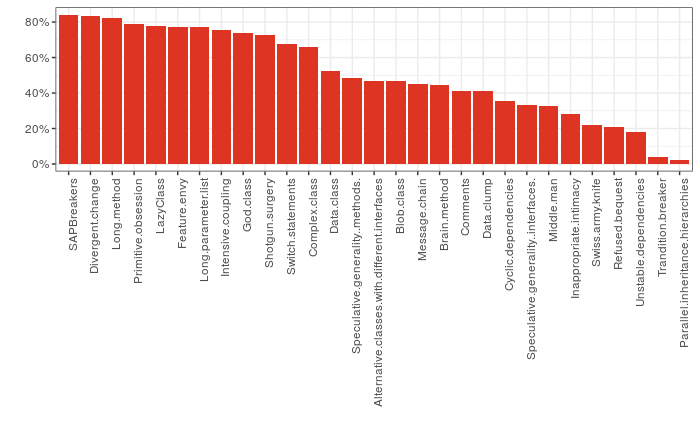
\includegraphics[scale=0.8]{figures/applications_contains_x_3.png}
    \caption{How many applications contain code smell $X$?}
    \label{fig:applicaitons_contain_x}
\end{figure}

Figure~\ref{fig:distribution}, displays distribution of detected code smells inside analyzed applications.

Here we can see that \say{Divergent change} makes up a significant part of the distribution which makes up to
$28\%$ (30718 detections) of total detected code smells.
It is followed by the \say{SAPBreakers} with detection rate of $9\%$ (10341) detections and \say{Long method}
with detection rate of $8.6\%$ (8343 detections).

The least frequent code smells, excluding \say{Missing Template Method} due to the fact that it has 0 detections,
are the following: \say{Unstable dependencies} with detection rate of $0.9\%$ (109 detections total),
\say{Parallel inheritance hierarchies} with detection rate of $0.6\%$ (70 detections total) and
\say{Tradition breaker} with detection rate of $0.1\%$ (17 detections total).

\begin{figure}
    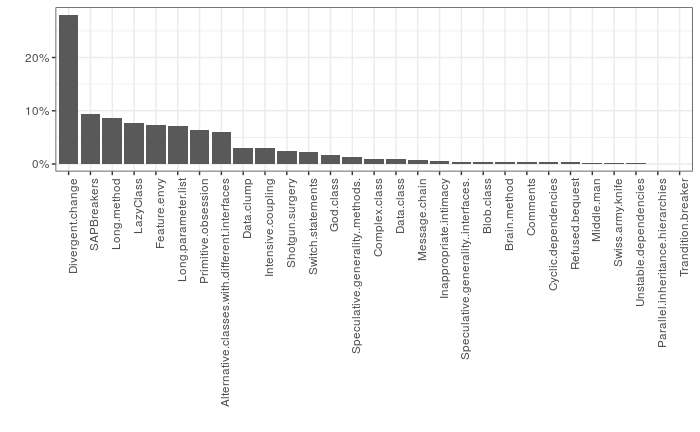
\includegraphics[scale=0.8]{figures/distribution_3.png}
    \caption{Distribution of code smells inside the analyzed applications.}
    \label{fig:distribution}
\end{figure}

\FloatBarrier

